\section{Architecture}
Fundamentally, the Common Language Runtime is a bytecode virtual machine that sits on top of an object-oriented type system.
Execution is represented as transferring control between the bodies of methods defined by parent types.
These method bodies are written in Common Intermediate Language (CIL), the bytecode instruction set defined by the ECMA-335 standard.
Each call to a method generates a new call frame that includes a stack, and the CIL uses this stack as ``scratch space'' for computation.
In addition to standard instructions such as arithmetic, branching, and basic stack manipulation, the CIL has a separate set of
``object model'' instructions that govern the construction of class objects, the handling of virtual method calls,
and loading/storing values in object fields. For details, see Appendix~\ref{app:cil}.
% TODO

\subsection{The Virtual Execution System}
The standard formally defines the semantics of CIL execution with the Virtual Execution System (VES) abstract machine.
The specifications

\subsubsection{Call frames}
Call frames and method state are explicitly specified as a component of the VES.
In particular, the ECMA standard specifies that each method keeps track of its own state (the current instruction pointer,
local variables/arguments, the evaluation stack, etc.) independently and the only data shared between methods is the garbage-collected heap,
as shown in Figure~\ref{fig:ves}.

\begin{figure}[h]
    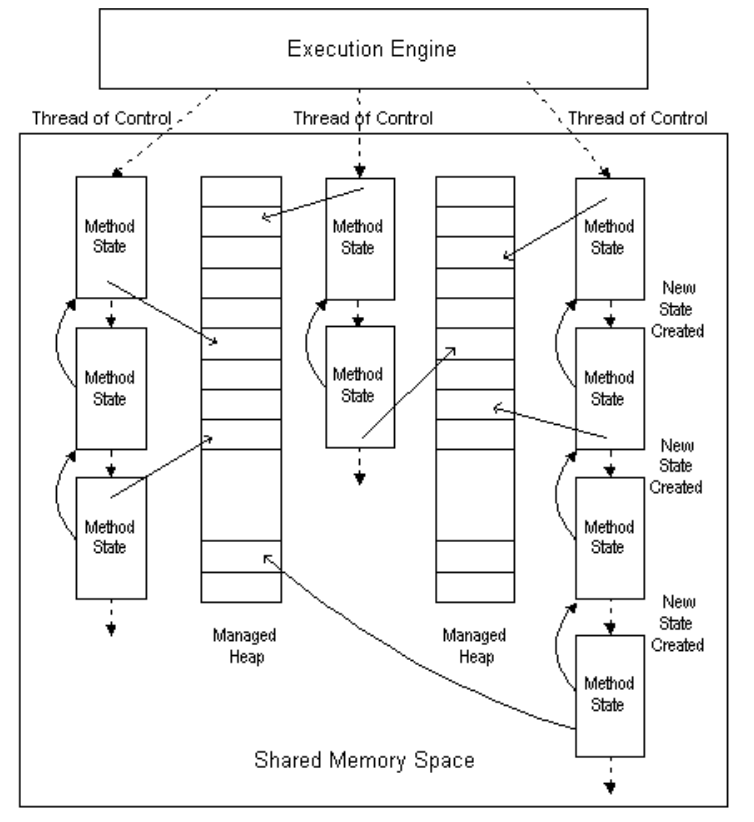
\includegraphics[width=3in,keepaspectratio]{ves}
    \centering
    \captionsetup{justification=centering}
    \caption{The structure of the VES and its nested method states, as represented by the ECMA standard~\cite{ecma335}.}
    \label{fig:ves}
\end{figure}

\subsubsection{Value storage}
The VES is not a ``true'' stack machine in the sense that all program information is stored on the stack;
rather, a method's stack is only a space to hold temporaries and set up arguments for method calls.
Instead, values are stored either in a method's declared local variables or within fields of an object.
These can be loaded onto the stack or stored from a stack value with the \texttt{ldarg}/\texttt{starg} and \texttt{ldfld}/\texttt{stfld}
CIL instructions.

At this point, the distinction between a full CLI value and a stack value becomes relevant.
While a CLI value can be an instance of an arbitrarily complex class or value type, a pointer, or a specific integer/floating-point type
(see section~\ref{sec:cts}),
the standard only requires that the evaluation stack support the following types as values:
\begin{itemize}
    \item 4-byte and 8-byte signed integers
    \item A pointer-sized signed integer
    \item A floating point value of unspecified precision
    \item Managed and unmanaged pointers (i.e., a pointer that references managed heap memory versus one known not to point into the heap)
    \item A GC-tracked reference to a CLI object
    \item User-defined value types
\end{itemize}
All other values are then transparently synthesized by the VES; for instance, a 1-byte integer will be zero-extended or sign-extended (as appropriate)
when loaded onto the stack, and CIL instructions that call specifically for 1-byte integers will have their arguments truncated.

\subsection{The Common Type System}\label{sec:cts}

\section{Implementation}

\subsection{Garbage collection with \texttt{gc-arena}}

\subsection{The call stack}

\subsection{CIL instructions}

\subsubsection{Unsafe operations}

